\documentclass{article}
\usepackage{graphicx} % Required for inserting images
\usepackage{parskip}

\title{Reddit Post Generator: Emulating Subreddit-Specific Style in Text Generation Using Mistral 7B}

\author{%
  \begin{tabular}{cc}
    Mauryan Uppalapati & Russell George \\
    Department of Computer Science & Department of Computer Science \\
    Tulane University & Tulane University \\
    \texttt{muppalapati@tulane.edu} & \texttt{rgeorge7@tulane.edu}
  \end{tabular}
}

\date{May 2024}

\begin{document}

\maketitle

\section{Abstract}
A platform such as Reddit has unique and very distinguishable linguistic styles.This provides both an opportunity and challenge for text generation using Large Language Models (LLM's).LLM's often fail at emulating these subreddit specific styles and instead produce text that is very generic.Our goal was to produce a model that given any topic and subreddit, would generate a post about that topic and that subreddit's style that would be indistinguishable from an actual reddit users post.Our project therefore attempted to develop "Reddit Post Generator", a model that utilises the Mistral 7B model fine-tuned on a dataset that was made up of ten distinct,text-based subreddit that would generate titles and posts that mimic the unique style and sarcasm unique to each subreddit.We use evaluation  metrics such as BLEU and human assessments to gauge the style accuracy of the generated texts. We found that while our model can accurately capture subreddit-specific styles , generating indistinguishable texts is still very challenging, especially under stress tests involving off-topic prompts.

\section{Introduction}
Online platforms like Reddit have a vast array of linguistic styles,where even each subreddit has its own unique style and sarcasm.These differences are not small but are actually central to the very identity of each community.Although there have been tremendous advances in Large Language models, they often are not effective in these context-rich environments.In data-rich scenarios there are lots of examples of LLM's that are good at learning language nuances but they struggle with the brief and topic-diverse nature of these Reddit posts.

The importance of accurately capturing these subreddit-specific styles goes beyond simple text generation. This emulation can be extrapolated to creating more engaging and personalized chatbot interactions. User engagement can also be boosted through the generation of tailored material and this could even enable  AI-driven moderation tools that can grasp the context of community discussions.This precise style emulation could lead to technologies that are capable of mimicking human-like interactions more convincingly. This could be very useful for applications such as digital assistants and social media management tools.

However, the capabilities of modern LLMs can often fall short. While they can generate grammatically correct text, they fail to capture the authentic tone and stylistic nuances that are specific to subreddits.

Therefore, we have developed the "Reddit Post Generator," which aims to produce content that is indistinguishable from posts written by real Reddit users. We aim to broaden the use of LLM's in personalized text generation tasks, ultimately aiming to enhance user interactions in digital spaces.

\section{Background/Related Work}
\vspace{10pt}

The paper \textit{A Feasibility Study of Prompt-enabled Text Stylization with Off-the-Shelf LLMs} by Bhandarkar et al. looks at the potential of using pre-trained Large Language Models for emulating individual author styles through strategic prompt engineering. The paper shows that while LLMs show promise in adapting to specific nuances of authors, they often times cannot  fully capture the depth and complexity of personalized writing styles. This paper goes to show the challenges and limitations of current LLMs in achieving the desired nuanced style emulation and also bring to light the  importance of prompt design to guide the stylistic direction of the generated text.

Our project the ``Reddit Post Generator,'' is somewhat similar but shifts the focus from individual authors to the distinctive styles of Reddit subreddits. THese author style studies have extensive datasets while our project deals more with brief and diverse data of subreddit posts, which can vary widely in style and content even within a single community. 
\vspace{10pt}


The paper \textit{How Well Can LLMs Echo Us? Evaluating AI Chatbots' Role-Play Ability with ECHO} looked into the capabilities of Large Language Models (LLMs)  to mimic average ordinary individuals rather than well-known or fictional characters, They used a framework called ECHO which was inspired by the Turing test to assess its abilities. This was good background for our project, the ``Reddit Post Generator,'' as we also want ti make AI-text seem more real  but instead focuse more on  the unique linguistic styles of differnt Reddit communities. The ECHO study used direct human feedback from friends to evaluate the human-likeness of responses whereas our project uses different evaluation metrics. 
\vspace{10pt}

The study \textit{Simulating H.P. Lovecraft horror literature with the ChatGPT large language model} by Garrido-Merchán et al. looks into the application of GPT-4 for emulating H.P. Lovecraft's unique literary style. The researchers here used advanced prompt engineering to replicate Lovecraft's stylistic elements. They also conducted surveys where participants could not reliably distinguish between AI-generated texts and genuine Lovecraft literature. This  approach gave us some insights on prompt engineering for our project, although we aimed to capture the diverse styles of various Reddit communities. We thought adapting their prompt engineering strategies could enhance our model's ability to  mimic the characteristics of different subreddits, and therefore improving the generated content.
\vspace{10pt}

The paper \textit{Mistral 7B: A High-Performance, Efficient Language Model} is an overview of the Mistral 7B model.It touches upon the attention mechanisms .We used this as background as in our project as we utilize the Mistral 7B model for generating the subreddit-specific posts.This helped us better understand the architecture of the model we planned to use.

\vspace{10pt}

The paper \textit{Prompting Large Language Models for Topic Modeling} introduced an approach that utilizes large language models (LLMs) for topic modeling at the sentence level. In our project, the data we used to generate subreddit-specific posts from Reddit data only had titles and bodies, therefore we needed a method to label topics. This paper gave us some insights into various topic modeling methods we could incorporate.

\section{Approach}

Our approach to  generate subreddit-specific posts started first by fine-tuning the Mistral 7B model 

\subsection{Data Collection}
We scraped data using the Python Reddit API Wrapper (PRAW), for the ten distinct subreddits. Each subreddit was chosen based on its unique style and the fact that they were mainly text based. The scraped data included only the titles and bodies of posts.

\subsection{Data Preparation and Formatting}
The data required careful preparation and formatting for the fine-tuning process. We cleaned the text to remove any non-relevant characters and formatted each entry to include both the subreddit name and the body.Since no other topic modelling method seemed to be effective we hand labelled twenty posts from each subreddit. This format allowed the Mistral 7B model to learn not just the language style of each subreddit but also how the topics are typically discussed within those communities.

\subsection{Model Fine-Tuning}
The fine-tuning of the Mistral 7B model was performed on the prepared dataset. The model was trained to generate both titles and bodies of posts based on a given subreddit and a topic. 

\subsection{Variation in Topic Inputs}
To explore the model's adaptability and creativity, we experimented with three types of topic inputs:
\begin{itemize}
    \item \textbf{Dataset-specific topics:} Topics that are commonly found within the subreddit data.
    \item \textbf{Common topics:} Popular topics across various subreddits, to test the model's ability to adapt the topic to different subreddit styles.
    \item \textbf{Edge case topics:} Unrelated or unusual topics for a given subreddit to see the model's capability in handling unexpected content.
\end{itemize}

\section{Experiments}

\subsection{Experimental Setup}
We wanted to test two different text generation methods: prompt-based and text completion-based generation. The same dataset, scraped from ten distinct subreddits, was used for both methods, although the data formatting varied between the two.

\subsubsection{Data Formatting}
For the prompt-based model, data was formatted using the "alpaca prompt format" which included structured instructions. Each row of the dataset consisted of:
\begin{itemize}
    \item Instruction: "Given the topic and subreddit, generate a title and body for a post."
    \item Input: The topic and subreddit.
    \item Output: The corresponding title and body.
\end{itemize}

The text completion model's dataset was formatted to contain the topic, subreddit, title, and body sequentially in each row, without explicit instructions. We wanted the model's inherent understanding to prompt the generation

\subsection{Generation Methods}
\begin{enumerate}
    \item \textbf{Prompt-Based Generation:} The model received the full instruction along with the topic and subreddit, it then generated the title and body.
    \item \textbf{Text Completion Generation:} This model was only given the topic and subreddit and then was tasked with generating the output.
\end{enumerate}

\subsection{Stress Testing}
Three types of topics were tested across all ten subreddits:
\begin{itemize}
    \item Dataset-specific topics
    \item Common topics across subreddits
    \item Edge case topics unrelated to the subreddit
\end{itemize}
These scenarios allowed us to perform comprehensive stress testing of the models, particularly evaluating how they handle unexpected content through edge case topics.

\subsection{Evaluation Metrics}
Both models were evaluated based on their BLEU scores. We measured how closely the generated text matched the human-generated posts from the same subreddits.

\section{Results}
The prompt-based model performed better on dataset-specific and common topics with it having an average BLEU score that was 44percent better. The text completion model showed varied results, especially in edge cases,sometimes even generating words in german that didnt appear in the dataset.(Look at evalresults file for more)

\section{Conclusion}

Our original goal was to create a Reddit Post Generator capable of mimicking the style and content of actual subreddit-specific posts,although we were well short of that mark.We really understood the importance of dataset preparation and formatting in fine-tuning language models for specific tasks.This taught us a lot about using and fine-tuning models for personalized tasks.Our future ideas would be to refine prompt engineering techniques and exploring some sophisticated attention mechanisms which could be beneficial for this task.

\section{References}

https://aclanthology.org/2024.personalize-1.6/
https://arxiv.org/html/2404.13957v1
https://arxiv.org/abs/2305.03429
https://arxiv.org/abs/2310.06825
https://arxiv.org/abs/2312.09693


\section{Screenshots}
\begin{figure}
    \centering
    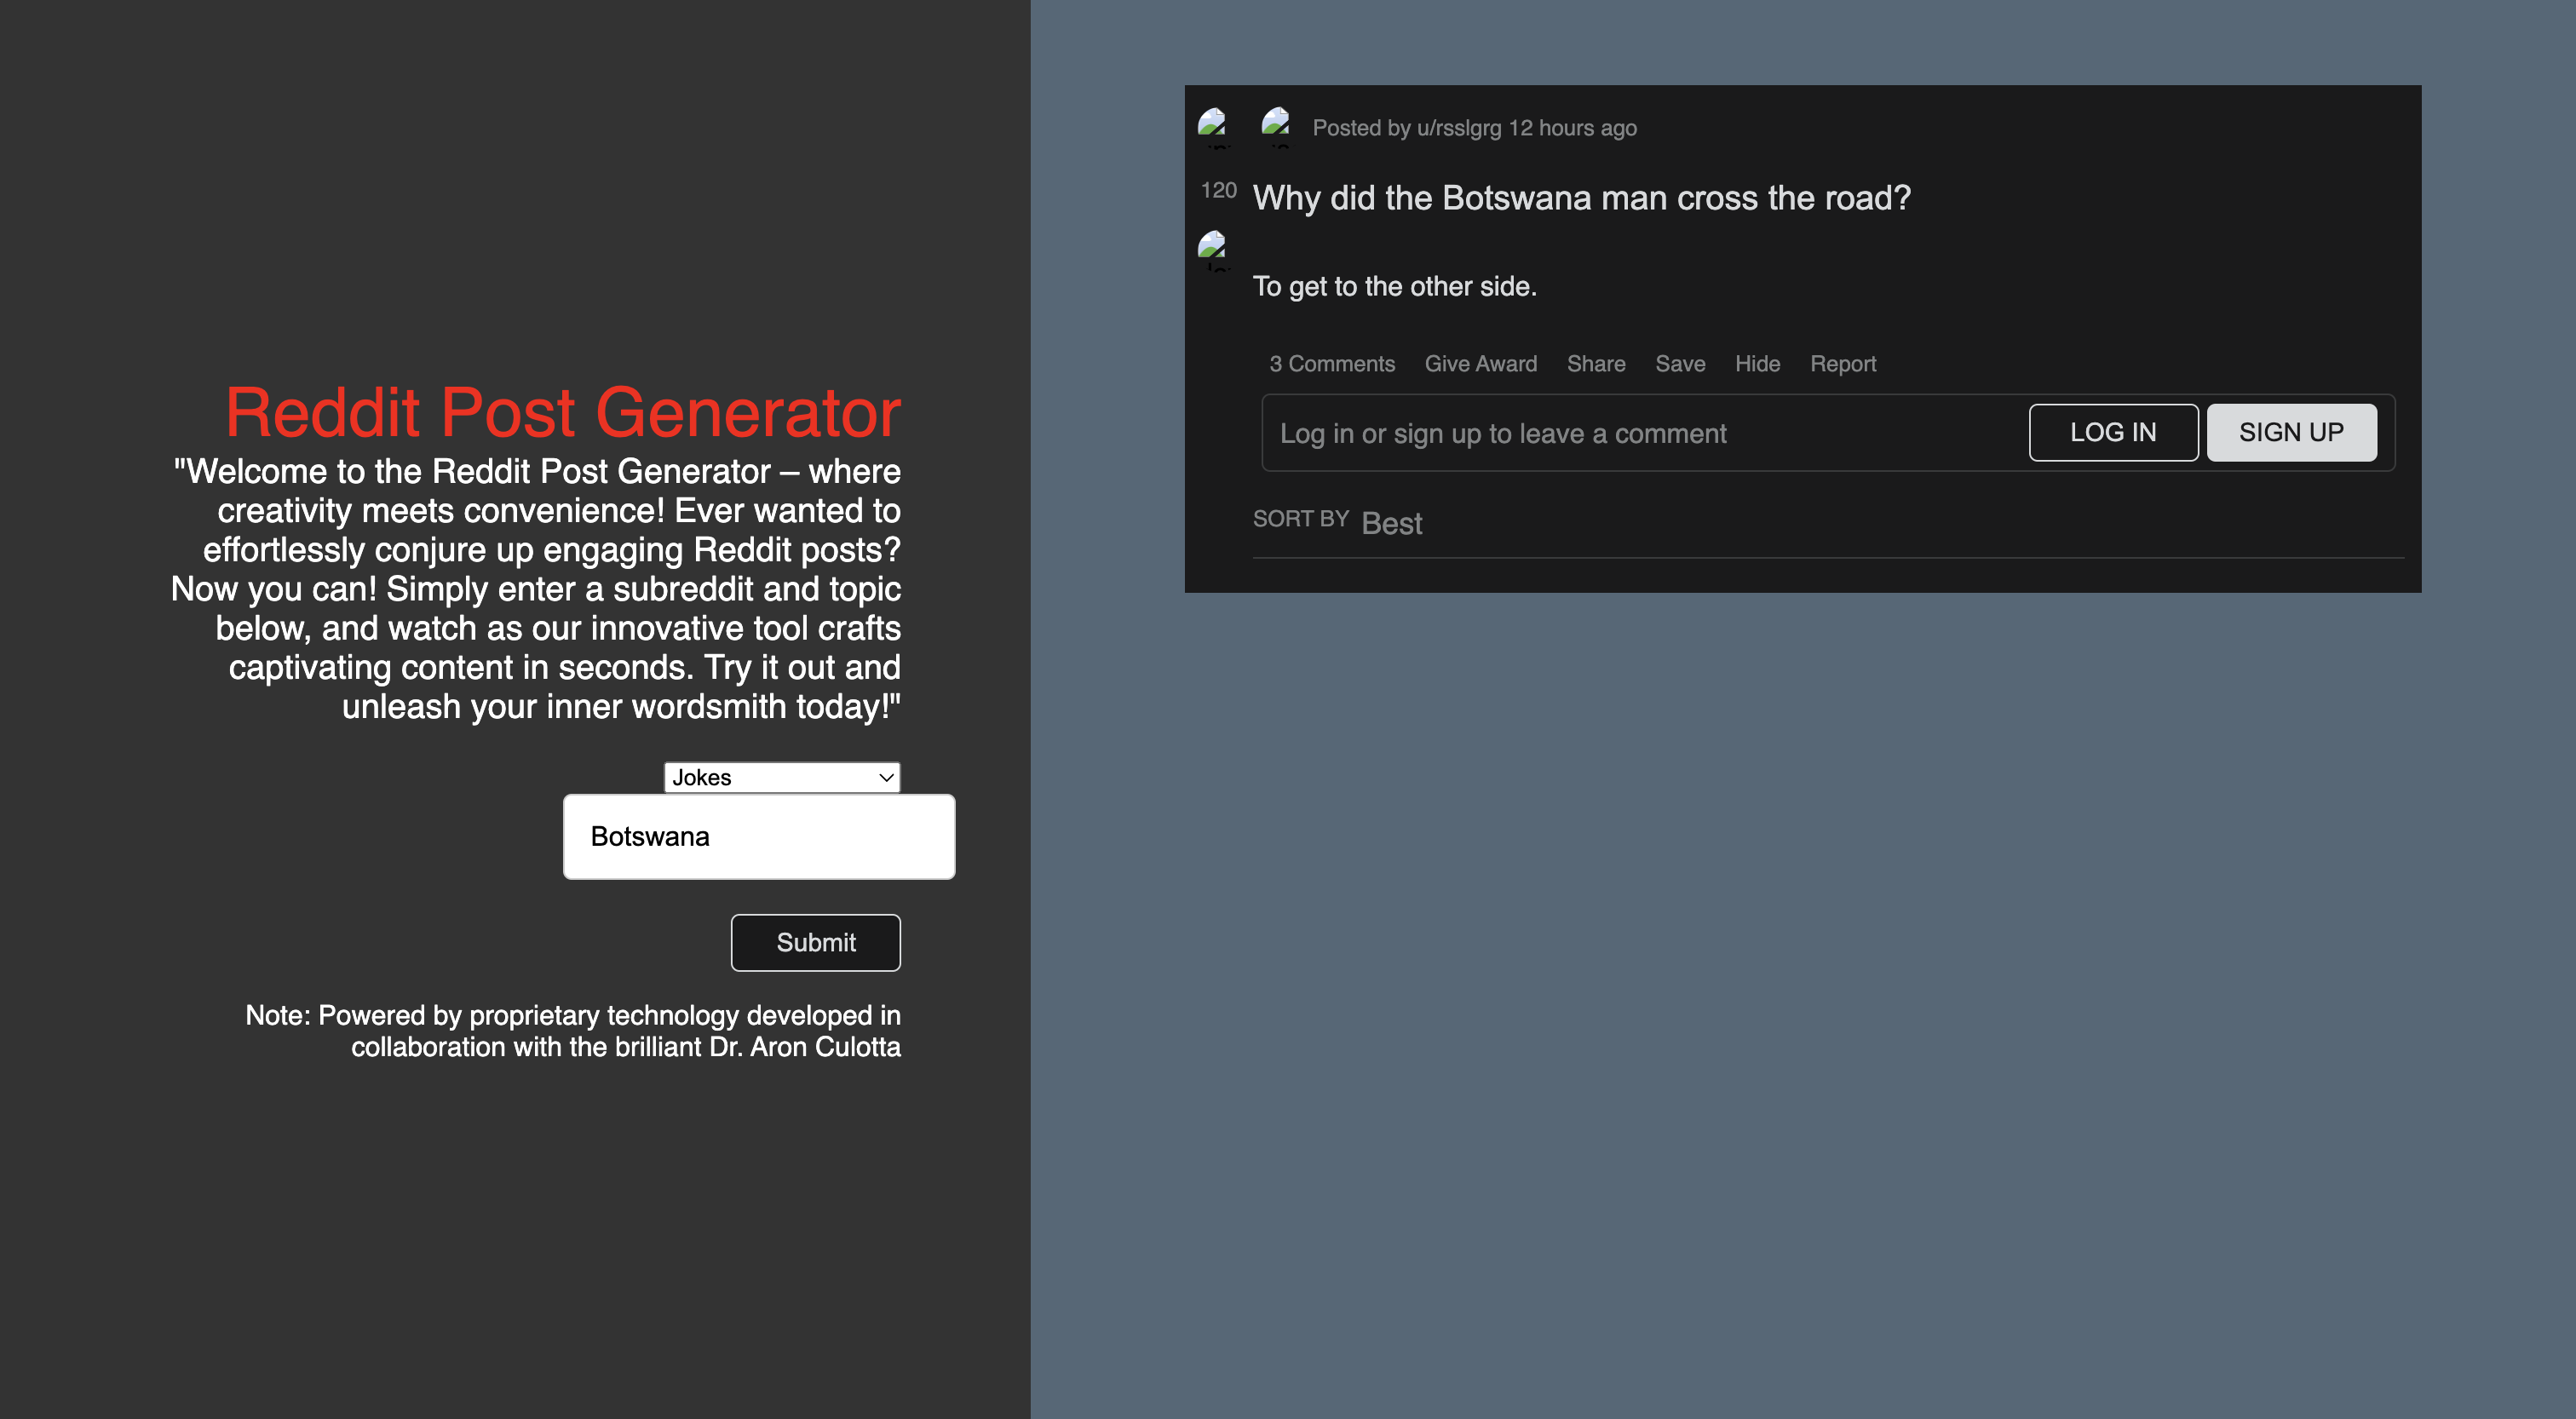
\includegraphics[width=0.5\linewidth]{bj-p.png}
    \caption{Demo}
    \label{fig:enter-label}
\end{figure}

\begin{figure}
    \centering
    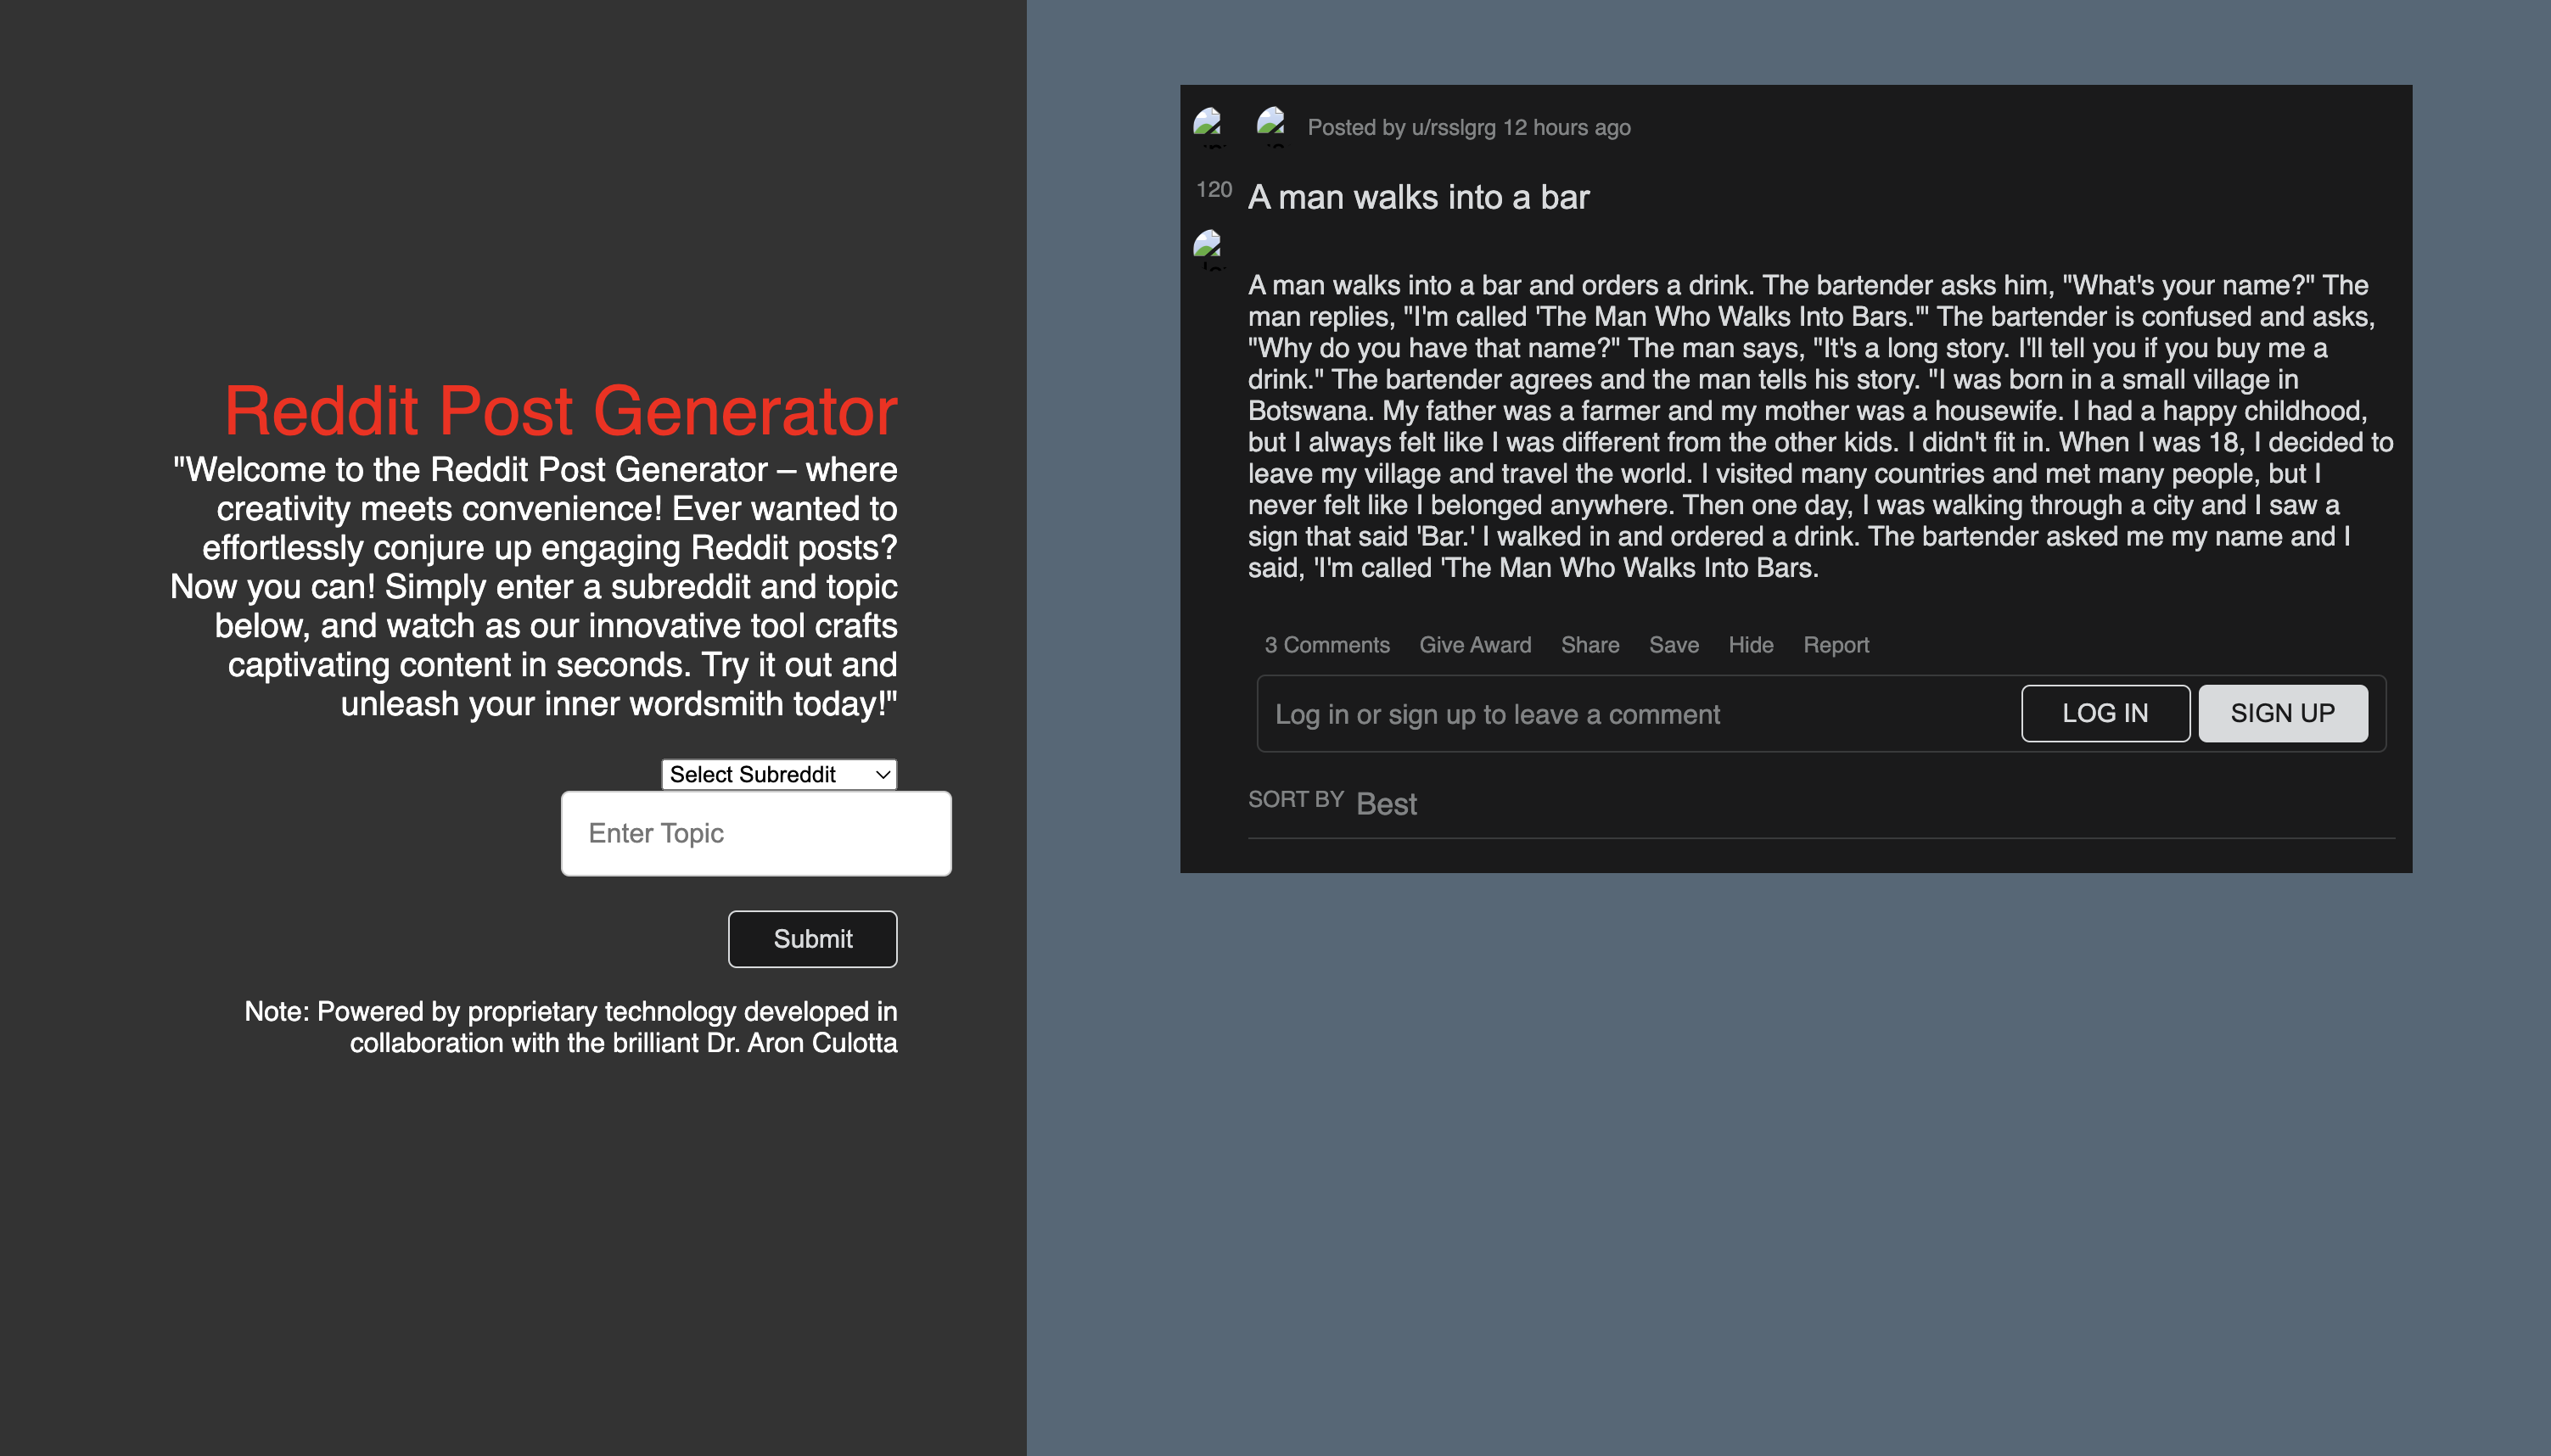
\includegraphics[width=0.5\linewidth]{bj-txt.png}
    \caption{Demo}
    \label{fig:enter-label}
\end{figure}



\end{document}
